\documentclass[english, 10pt]{article}
% \usepackage{amsmath}
\usepackage[sexy]{evan}
\usepackage{inconsolata}
\usepackage[shellescape]{gmp}
\usepackage{titlesec}
\usepackage{color}
\usetikzlibrary{arrows.meta}
\definecolor{editorGray}{rgb}{0.95, 0.95, 0.95}
\definecolor{editorOcher}{rgb}{1, 0.5, 0} % #FF7F00 -> rgb(239, 169, 0)
\definecolor{editorGreen}{rgb}{0, 0.5, 0} % #007C00 -> rgb(0, 124, 0)
\usepackage{listings}
\usepackage{xcolor}
\usepackage[toc,page]{appendix}
\usepackage{todonotes}
\usepackage{blindtext}
\usepackage{multicol}
\usetikzlibrary{calc,shapes.multipart,chains,arrows}
\usepackage{esint}
\usetikzlibrary{shapes.multipart}


\definecolor{dkgreen}{rgb}{0,0.6,0}
\definecolor{gray}{rgb}{0.5,0.5,0.5}
\definecolor{mauve}{rgb}{0.58,0,0.82}

\lstset{frame=tb,
  language=R,
  aboveskip=3mm,
  belowskip=3mm,
  showstringspaces=false,
  columns=flexible,
  basicstyle={\small\ttfamily},
  numbers=none,
  numberstyle=\tiny\color{gray},
  keywordstyle=\color{blue},
  commentstyle=\color{dkgreen},
  stringstyle=\color{mauve},
  breaklines=true,
  breakatwhitespace=true,
  tabsize=3
}

\allowdisplaybreaks%
\renewcommand{\O}{\mathcal{O}}
\newcommand{\thiscoursecode}{STAT 400}
\newcommand{\thiscoursename}{Applied Statistics and Probability I}
\newcommand{\thisprof}{Prof. Paul J. Smith}
\newcommand{\me}{Elizabeth Qiu}
\author{Elizabeth Qiu\thanks{Email: \mailto{elizabethjqiu@gmail.com}}}
\newcommand{\thisterm}{Summer 2022}
% \newcommand{\website}{https://www-math.umd.edu/offered-courses/412-stat-400-applied-probability-and-statistics-i.html}%chktex 8
\usepackage{ifpdf}
\ifpdf%
\DeclareGraphicsRule{*}{mps}{*}{}
\fi
\lhead{\textbf{\me} \\ \textbf{\thisprof}}
\rhead{\textbf{\thiscoursename} \\ \textbf{\thisterm}}

\newcommand{\notefront}{%
\pagenumbering{arabic}
\begin{center}
{\small}
\textbf{\Huge{{\thiscoursecode}}}
{\Huge \par}
{\Large{{\thiscoursename}}}\\
\vspace{0.1in}
\vspace{0in}
\includegraphics[scale=0.1]{media/umd.png} \\
\vspace{0.1in}{\me} \\
{\thisprof} \ $\bullet$ \ {\thisterm} \ $\bullet$ \ {{University of Maryland}} \\
{\ttfamily \url{\website}} \\
\end{center}
}

\begin{document}
\thispagestyle{empty}
\notefront
\tocandfigures

% wk1
\section{Monday, July 11, 2019}
This class is STAT400: Applied Probability and Statistics I. Topics covered: random variables, standard distributions, moments, law of large numbers and central limit theorem, sampling methods, estimation of parameters, testing of hypotheses.

\subsection{Logistics}
\begin{itemize}
	\item Textbook: Devore (2018), Probability and Statistics for Engineering and the Sciences ($9th\%$ ed). Cengage Learning.
    \item All lectures are recorded and posted on Panopto.
    \item No collaboration on projects.
    \item Frequent homework assignments and possibly pop quizzes. Assignments on ELMS.
    \item Assignments on ELMS. 
    \item The grade breakdown is $10\%$ for Homeworks, $10\%$ for Quizzes, $25\%$ for 2 Midterms $1$, and $40\%$ for the Final Exam. 
\end{itemize} 

\subsection{Probability, Statistics and Data}
In STAT400, we will visualizing and summarize data, and also use mathematical methods for data analysis.
\begin{enumerate}
	\item \vocab{Statistics} is the science of recognizing, collecting, analyzing, interpreting data.
    \item \vocab{Probability} is the mathematical theory of randomness and most of this course will be devoted to modeling random phenomena. 
	\item \vocab{Randomness} is a type of abstraction in which various data objects are known to the user, but how they are represented or implemented is not known to the user. An example of data abstraction is shown by representing a list of people. While the user would know that they have a list of people, they wouldn't know how the list is being represented (for example, we could use an array, an ArrayList, or any other data structure).
\end{enumerate}

## We went over the "Newcomb's 1882 Measurements" example, where measurements of the passage time of light were recorded by NewComb in 1882. Given values divided by 1000 plus 24 give the time in microseconds for light to traverse a known distance. We had a dataset with a summary of a minimum, 1st quartile value, median, mean, 3rd quartile value, maximum value, and standard deviation.


Once we have the central value of the data: "how close/far do we expect the values to be?"
Later: standard deviation: value that tells you how close/far away from typical observation we see data / absval of typical distance from mean
Histogram: good for visualizing data, shape of graph tells you typical distributions
Outliers: outside of bulk of data

Interpreting histograms:
- Values that are clearly separated from others = outliers
- Roughly follow "bell curve". Low ends of scales, maximum near mean or median. Bell shapes are not recognized without the graph
- Dropping outliers: only slightly change the mean and median, but may greatly affect standard deviation (outliers affect spread greatly)

Comparing samples graphically: histograms give good viz of shape/distributions
\vocab{Boxplot} = we take the min observation, max observation, lower and upper lines are 1st and 3rd quartiles, heavy line in middle is median. Whiskers (horizontal lines) measure spread: interquartile range.
Boxplot of a single sample is not really that useful, especially where calculations can be made instantly with a couple lines of code. But it's just as easy to create a histogram.
Don't worry too much about Count Data.
Most data we will encounter in this course is Measurement Data.

## Cereals
Histograms are not a reliable indicator when you have small samples of data, like we have in this example.

Recommended: Learn R. You can also use R to analyze data. It's free!



\subsection{The Java Programming Language}
Different programming languages provide varying levels of support for object-oriented programming. In particular, Java and C++ allow us to easily perform object-oriented programming. How does Java does this?
\begin{itemize}
    \item Java provides us with \vocab{interfaces}, which allows us to specify a set of methods that another class must implement. This allows us to easily express an abstract data type since we can specify the operations and data that an entity must have. Interfaces follow an ``is-a" relationship, meaning that a class that implements an interface is what the interface specifies. As an example, consider an animal interface. If an elephant implements the animal interface, we can perform tasks that are meant for animals with elephants (such as passing an elephant into a function that accepts animals). 
    \item Java provides us with \vocab{classes}, which can be used as blueprints for other classes. Classes can extend other classes, which makes them \vocab{subclasses}. These subclasses inherit functions from the original class, and this also defines an ``is-a" relationship. 
\end{itemize}

Here are some key points that we should remember about interfaces:
\begin{itemize}
    \item An interface cannot be instantiated. So, if we have an interface called \verb!animal!, typing \verb!Animal a = new Animal()! \textbf{would not compile}.
    \item An interface can contain many public members, including static final constants, abstract methods (which have no body), default methods (with a body), static methods, and static nested types.
\end{itemize}

Let's look at an example of an interface:

\begin{lstlisting}
    import java.util.*;

    public interface Animal {
        
        public void feed(String food);
        public int getAge();
        public boolean manBestFriend();
        
        default void grow() {
            System.out.println("I grow");
        }
    }
\end{lstlisting}

Here, we've created an interface named \verb!Animal!, which other classes can implement. Any class that implements this class will need to also implement the functions \verb!feed!, \verb!getAge()! and \verb!manBestFriend()! with the same return values and parameters specified. The \verb!grow()! function will be associated with any class that implements this interface.

Now let's look at another class that implements the \verb!Animal! interface:

\begin{lstlisting}
package animalExample;

public class Dog implements Animal {
	private String name;
	private int age;

	public Dog(String name, int age) {
		this.name = name;
		this.age = age;

	}

	public void feed(String food) {
		System.out.println("Feeding " + name + " with " + food);
	}

	public int getAge() {
		return age;
	}

	public boolean manBestFriend() {
		return true;
	}

	public void bark() {
		System.out.println(name + " is barking");
	}
}
\end{lstlisting}

Here are the key things that we should note:
\begin{itemize}
    \item The \verb!Dog! class implements the \verb!Animal! class. Thus, it is \textbf{required} to implement all of the methods specified by \verb!Animal! (if we were to comment out even one function, the code wouldn't compile).
    \item The \verb!Dog! class is allowed to add its own methods, like \verb!bark()!. Likewise, the \verb!Dog! class is allowed to create its own variables, like \verb!name! and \verb!age!.
\end{itemize}

Here's another class that implements the \verb!Animal! interface:

\begin{lstlisting}
package animalExample;

public class Piranha implements Animal {
	private int age;

	public Piranha(int age) {
		this.age = age;
	}

	public void feed(String food) {
		System.out.println("Piranha is eating " + food);
	}

	public int getAge() {
		return age;
	}

	public boolean manBestFriend() {
		return false;
	}

	public void grow() {
		System.out.println("I grow like a fish");
	}
}
\end{lstlisting}

Here are some more things that we should take careful note of: \begin{itemize}
    \item More than one class can implement an interface. In this example, both \verb!Dog! and \verb!Piranha! implement \verb!Animal!.
    \item We can rewrite methods that are provided to us. More specifically, \verb!Piranha! implements \verb!Animal!, but it rewrites the \verb!grow()! function that was originally provided to it.
\end{itemize}

Recall that interfaces define an ``is-a" relationship. Since \verb!Piranha! and \verb!Dog! implement \verb!Animal!, we can now treat them as an \verb!Animal!. A good way to verify the ``is-a" relationship is the \verb!instanceof! keyword. In Java, \verb!instanceof! allows us to check whether one object is an instance of a specified type (class, subclass, or interface).

To demonstrate, suppose we declare a piranha variable \verb!p!. We could write a conditional such as \verb!if (p instanceof Animal) { /* Code to be executed */}!, in order to make sure that \verb!p! is an instance of \verb!Animal!. Why would we ever need to do this? This is particularly useful when we're casting. If we attempt to cast an object to a subclass of which it is not an instance of, Java throws a \vocab{ClassCastException}. We can prevent this exception by putting the relevant code in a conditional checking the instance of what we're casting. %
\section{Tuesday, July 12, 2022}

\subsection{Probability Calculations}
Events can be combined ``algebraically" using unions, intersections and complements. There must be corresponding arithmetic rules for calculating their probabilities. These rules are all derived from the axioms. We need to assign probabilities for any theoretical or real-world situation.

For example, we might define the success probability on any trial by $p$ and the failure probability by $1-p$, regardless of what happens on other trials. Then a sequence \{SFSS\}, where $S$ is a success and $F$ is a fail, is assigned probability $p^3(1-p)$.\\

Basic Formulas
\begin{itemize}
    \item As we have seen, the sample space $S$ is an event with probability 1. Its complement is the empty set $\varnothing$. Therefore, $S$ is the certain event and $S^\mathsf{'} = \varnothing$ is the impossible event. If $A$ and $B$ are disjoint, then $A \cap B = \varnothing$.
    \item Here are some basic formulas, proved in the text: $$P(A) = 1-P(A^\mathsf{'})$$
    $$P(A \cup B) = P(A) + P(A\mathsf{'} \cap B)$$
    $$ = P(A) + [P(B) - P(A \cap B)]$$
    $$ = P(A) + P(B) - P(A \cap B)$$
    $$P(A \cup B \cup C) = P(A) + P(B) + P(C) - P(A \cap B) - P(A \cap C) - P(B \cap C) + P(A \cap B \cap C)$$
\end{itemize}
\begin{itemize}
    \item ``In general, the probability of a union of $k$ events is obtained by summing individual event probabilities, subtracting double intersection probabilities, adding triple intersection probabilities, subtracting quadruple intersection probabilities, and so on" (page 63, \cite{devore}).
    \item If $A$ occurs whenever $B$ occurs, then $A$ is a \vocab{subset} of $B$, written $A \subseteq B$. In words, $A$ \textit{implies} $B$. Other interpretation include: ``is contained in''. In this case, ${P(A)} \le {P(B)}$.
    \item If $S$ is a certain event that will occur, then the complement of $S$ is an impossible event. Two disjoint events’ intersection is an empty set (because it will be impossible that those two events will occur at the same time).
    \item Formulas like these are suggested by Venn diagrams but are proved using the axioms.
\end{itemize}
Assigning Probabilities
\begin{itemize}
    \item One must know the sample space and the form of the outcomes.
    \item Let $S = {S_{1}, S_{2}, \ldots, S_{m}}$. Choose numbers $p_{j}, j=1, \ldots, m$ such that $0 \le p_{j} \le 1$ (you choose the probabilities for each $p_{j}$) and $\sum_{j=1}^{m}p_{j}=1$. In this setup, any event has finitely many outcomes. Its probability is the sum $$P(A)=\sum_{s_{j}\in A}p_{j},$$ where each outcome belongs to $A$, with a probability $p_{j}$ attached to it. This rule is used in gambling games with equally likely outcomes.
    \item Thinking concept for probability in terms of size of a geometric region: if $S$ is a geometric region and $A$ is a subregion, we can define $P(A) = \frac{size\,of\,A}{size\,of\,S}$. ``Size" might mean length (of a line segment), area (of a plane region), or volume (of a solid). This only makes sense if $S$ is bounded.
\end{itemize}

\subsection{Counting}
Probability theory began in the 17th century with the analysis of gambling games, such as cards, coin tossing, dice, or roulette. Often a gamble might be repeated several times. Gambles usually have finitely many outcomes. If the gamble is fair, each outcome should have the same probability.

To calculate probabilities, one must calculate the number of outcomes in $S$, say $n$, and the number of outcomes in some event $A$, say $n_{A}$. Then, $P(A)=\frac{n_{A}}{n}$.

Small sample spaces can be counted explicitly. Then $P(A)$ can be calculated for any $A$. For larger and more realistic setups, it may be easier to imagine the experiment as conducted in steps.

\textbf{Example 1}: A committee of 2 members is chosen from an organization of 10 members. First a committee chair is selected; there are 10 ways to do this. Then, a secretary is chosen from the remaining 9 members. Therefore, there are $90 = 10\times9$ ways to select the committee.

\textbf{Example 2}: Two dice, one red and one green, are tossed. There are 6 outcomes for the red die and 6 for the green die. Therefore, there are $36=6\times6$ outcomes of the experiment.

The previous examples illustrate a general principle for a two-step process (assuming that each of the outcomes are equally likely). Suppose there are $m$ outcomes in the first step, followed by $n$ outcomes in the second step based on the outcome in the 1st step from $m$. Then, there are $mn$ total outcomes for the two step process. This principle can be displayed using a \vocab{tree diagram}, where each path through the tree is one way to perform the two-step process. It generalizes to $k$ step processes for any $k$.

\subsection{Permutations and Combinations}
Suppose there are $n$ objects (persons, households, etc.) and we want to select $k$ objects \textit{in order}. That is a \vocab{permutation}, or ordered arrangement. But how many permutations are there? We create the permutation in $k$ steps and use the basic principle:

\begin{enumerate}
    \item Choose the first object: there are $n$ ways.
    \item Choose the second object: there are $n-1$ ways.\\
    \vdots\\
    $k$. Choose the $k$-th object: there are $n-(k-1)$ ways. 
\end{enumerate}
Hence there are $n(n-1)(n-2)\hdots(n-(k-2))(n-(k-1))=\frac{n!}{(n-k)!}$ permutations (``$\text{permute}\,n\,k$").

A key assumption about permutations is that the objects are distinguishable. This is obviously true is one is permuting persons, but we can imagine that objects are distinguishable, as in \textbf{Example 2}.

But often, order of selection is not important. For example, in a political poll, order of selection is irrelevant. The only event of interest in a poll might be how many sampled persons will vote Democrat or Republican. A \vocab{collection} is an unordered set of $k$ objects chosen from a collection of $n$ objects. Imagine that the objects are names drawn simultaneously from a hat.
 
To count the number of combinations of $k$ objects chosen from a set of $n, C_{k,n}$, we imagine a two-step process:
\begin{enumerate}
    \item Choose a combination: $C_{k,n}$ ways.
    \item Arrange the elements of the combination in order: $k!$ ways.
\end{enumerate}

The result is a permutation of $k$ (size subset) out of $n$ objects (to choose from). Therefore (``$\text{choose}\,n\,k$"):
$$P_{k,n} = \frac{n!}{(n-k)!} = C_{k,n} \times k!$$
$$C_{k,n} = \frac{n!}{k!(n-k)!} = {n \choose k}$$

The $n \choose k$ (``$n \, \text{choose} \,k$") notation is more common, and $n \choose k$ is called a \vocab{binomial coefficient}, because it comes from the binomial theorem (to be discussed later). Note that ${n \choose n} = {n \choose 0} = 1$, and ${n \choose 1} = n$.

\subsection{Basic Counting Principle; Sampling and Replacement}
Polls and surveys select combinations of persons from a population. This is also true of many card games, such as poker. By contrast, gambling games like dice or roulette repeated trials where the outcomes are the same at each step.

The \vocab{basic counting principle} says that if each step in a multi-step experiment has $n$ outcomes, then there are $n^k$ outcomes in the combined experiment. Drawing without replacement results in $\frac{n!}{(n-k)!}$ outcomes, and drawing with replacement results in $n^k$ outcomes. Examples include lotteries, raffles, powerballs, etc.
\begin{enumerate}
    \item \textbf{Example 3}: Urn: Imagine an urn with balls numbered $1, 2, \ldots, n$. If we draw $k$ balls without replacement there are $\frac{n!}{(n-k)!}$ outcomes. If we draw a ball and replace it, there are $n^k$ outcomes.
    \item \textbf{Example 4}: Daily lotteries: A player bets on a three or four-digit number. There are $10^3$ or $10^4$ possible outcomes.
    \item \textbf{Example 5}: Raffles: Suppose 10,000 tickets are sold and there is a first prize, second prize, and third prize. Then, the winning tickets are a permutation of three tickets out of 10,000.
    \item \textbf{Example 6}: Powerball: A player bets on a permutation of 5 out of 69 numbers along with a powerball number, chosen from \{1, 2, \ldots, 26\}. There are $(69 \times 68 \times 67 \times 66 \times 65) \times 26$ outcomes.
\end{enumerate}

\vocab{Sampling without Replacement}, and \vocab{Ordered sampling with Replacement}\\

\textbf{Example 7}: Imagine an urn contains $r$ red balls and $b$ blue balls. If $k$ balls are drawn without replacement, find $P(A) = P(\text{exactly 4 red balls})$ (assuming equally likely outcomes). 

The sample space contains $r+b \choose k$ outcomes. If $A$ occurs, 4 of the $r$ red balls were chosen and $k-4$ of the blue balls were chosen. The red balls are a combination of 4 out of $r$ red balls. Similarly, the blue balls are a combination of $k-4$ out of $b$ blue balls.

Using the basic principle, the formula for combinations and the equally likely assumption, $$P(A) = \frac{{r \choose 4}{b \choose k-4}}{{r+b \choose k}}.$$

\textbf{Example 8}: Now assume $k$ balls are drawn from the urn \textit{with} replacement. This form of sampling automatically identifies a first, second, etc. ball. Now the sample space has $(r+b)^k$ possible outcomes. We want to find $P(B) = P(\text{first red ball on the fifth draw})$.

If $B$ occurs, the outcome must have been of the form $bbbbrxxx \ldots x$, where the sequence begins as shown, $b$'s are blue, $r$'s are red, and the $x$'s are colored arbitrarily. There are $b^4(r+b)^{k-5}$ outcomes in $B$. Therefore, $$P(B) = \frac{b^4r(r+b)^{k-5}}{(r+b)^k} (\text{the number of outcomes of $B$ divided by the sample space}) = \frac{b^4r}{(r+b)^5}.$$

If the sampling were ordered without replacement, then $$P(B)=\frac{[\frac{b!}{(b-4)!}]r}{[\frac{(r+b)!}{(r+b-4)!}]}.$$ A good application of ordered sampling without replacement is quality testing.%
\section{Wednesday, July 13, 2022}
Due to the power outages caused by the storm yesterday, there is no class today. Continue working on the assigned homework problems.%
\section{Thursday, July 14, 2022}
Due to the power outages caused by the storm on July 12, the professor's video and screensharing Zoom options were not available in class today. Instead, we went over a few questions students had.

Continue working on the assigned homework problems. Missing two days of instruction results in a missed week. We will probably cut off a small portion of chapter 7 content.%
\section{Friday, July 15, 2022}

\subsection{Conditional Probability}
\textbf{Example 1}: Political poll: A political poll is conducted in Maryland. Respondents are classified by resident (urban, suburban, rural) and party preference (Democrat, Independent, Republican). The results are recorded and treated as probabilities. Thus $P(\text{Democrat \& Rural}) = 0.03$, $P(\text{Suburban}) = 0.40$, $P(\text{Independent}) = 0.30$, etc.

A politician may be interested in the proportion of suburbanites $P(\text{Suburban}) = 0.40$ who are Republicans $P(\text{Republican \& Suburban}) = 0.03$. The proportion is $\frac{0.03}{0.40} = 0.075$.

The calculation $\frac{P(\text{Republican \& Suburban})}{P(\text{Suburban})} = 0.075$ is the \vocab{conditional probability} that a person is a Republican, given that they are a suburbanite. In symbols, $P(\text{Republican}|\text{Suburban}) = \frac{P(\text{Republican \& Suburban})}{P(\text{Suburban})}$. We are assuming that $S$ has occurred, and we see that the occurrence of $S$ changes the probability of being a Republican. This is because of the sample space changes from the whole state to suburbanites only.

The general definition is that for any two events $A$ and $B$ such that $P(B)>0$, $$P(A|B) = \frac{P(A \cap B)}{P(B)}.$$

This definition yields the \vocab{multiplication rule}: $$P(A \cap B) = P(A|B) \times P(B).$$

There is no one simple way to compute $P(A|B)$. In some cases we can calculate $P(A \cap B)$ and $P(B)$ directly (as in \textbf{Example 1}) and then we can easily evaluate $P(A|B)$ by division. In other problems, we think of $B$ as a new reduced sample space. If probabilities on $B$ are easy to compute, we evaluate $P(A|B)$ directly.

\textbf{Example 2}: Urn problem, revisited: As before the urn contains $r$ red and $b$ blue balls. Balls are selected one at a time without replacement. We want $P(B_{2}) = P(\text{blue ball on second draw})$. The first ball results in either $B_{1}$ or $B^\mathsf{'}_1 = R_{1}$, where $B_{1} = \{\text{blue ball on first draw}\}$.

From the problem, we can conclude that $P(B_{1}) = \frac{b}{b+r}$ and $P(B^\mathsf{'}_{1}) = \frac{r}{b+r}$. Now consider $P(B_{2}|B_{1})$. Think of $B_{1}$ as a reduced sample space with $r$ red and $b+r-1$ blue balls. Then, we see that $P(B_{2}|B_{1}) = \frac{b-1}{b-1+r}$. Similarly, $P(B_{2}|B^\mathsf{'}_1) = \frac{b}{b-1+r}$.

\vspace{0in}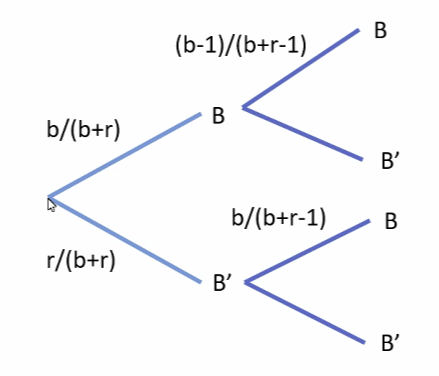
\includegraphics[scale=1]{media/wk1tree.png} \\

From Axiom 3, we see that $B_{2} = (B_{1} \cap B_{2}) \cup (B^\mathsf{'}_1 \cap B_{2})$ which is a union of disjoint sets. So $P(B_{2}) = P(B_{1} \cap B_{2}) + P(B^\mathsf{'}_1 \cap B_{2})$. The multiplication rule says that $P(B_{1} \cap B_{2}) = P(B_{1}) \times P(B_{2} | B_{1})$ and $P(B_{1} \cap B_{2}) = P(B_{1}) \times P(B_{2}|B_{1})$. We find that $P(B_{2}) = \frac{b}{b+r}$, which is identical to $P(B_{1})$. Drawing a tree to illustrate this scenario would also be helpful. 

\subsection{Total Probability}
Suppose $S$ is partitioned into subsets $A_{1}, A_{2}, \ldots, A_{k}$, which are disjoint. This means that $S = A_{1} \cup A_{2} \cup \cdots \cup A_{k}$ and $A_{i} \cap A_{j} = \varnothing$. In the venn diagram, $k=5$.

\vspace{0in}
\includegraphics[scale=1]{media/wk1totalprobability.png} \\

The white oval is the event $B$ and the rectangle is sample space $S$. The red lines indicate the partitioning sets $A_{1}, A_{2}, \ldots, A_{k}$. Note that $B$ is also partitioned into disjoint subsets $(A_{1} \cap B), \ldots, (A_{k} \cap B)$.

Now Axiom 3 yields the Total Probability Formula: $$P(B) = P(A{1} \cap B) + \cdots + (A_{k} \cap B) = \sum_{j=1}{k}P(A_{j}) \times P(B|A_{j}).$$

\textbf{Example 3}: Political poll, continued: In the example of the political poll, we can see that $P(\text{Democrat}) = P(\text{Democrat} \cap \text{Republican}) + P(\text{Suburban} \cap \text{Democrat}) + P(\text{Urban} \cap \text{Democrat}) = 0.03+0.25+0.32$.

\textbf{Example 4}: Friend mail: You ask a friend to mail a letter. They will forget to mail it (event $M^\mathsf{'}$) with probability 0.1. If it is mailed, the Post Office will fail to deliver the letter (event $D^\mathsf{'}$) with probability 0.1. With is $P(D^\mathsf{'})$? From the Total Probability Formula, $P(D^\mathsf{'}) = P(D^\mathsf{'} \cap M) + P(D^\mathsf{'} \cap M^\mathsf{'}) = (0.1)(0.9) + (1)(0.1) = 0.19$.

\subsection{Bayes' Formula}

In the setup of the Total Probability Formula, let $A_{j}$ be possible causes and $B$ be a result. We know $P(A_{j})$ and $P(B|A_{j})$ for $j = 1, \ldots, k$.

If we observe that $B$ occurs, we might ask, ``what is the chance that $B$ was caused by $A_{j}$?" In other words, what is $P(A_{j}|B)$?

The answer is \vocab{Bayes' Formula}: $$P(A_{j}|B) = \frac{P(A{j} \cap B)}{P(B)} = \frac{P(A_{j}) \times P(B|A_{j})}{\sum_{i}P(A_{i}) \times P(B|A_{i})}$$

Bayes' formula is an application of the Total Probability Formula.

\textbf{Example 5}: COVID-19 testing: A diagnostic test for disease, such as COVID-19, is characterized by two parameters: $\text{Sensitivity} = SE = P(+|D)$, and $\text{Specificity} = SP = P(-|D^\mathsf{'})$. Let $+=\text{testing positive}$, $-=\text{testing negative}$, and $D=\text{the patient has the disease}$.

However, the performance of the test also depends on the prevalence of disease in the population, i.e., $P(D)$.

Suppose $P(D) = 0.05$, $SE = 0.90$, and $SP = 0.95$. The real question is ``if a patient tests positive, do they really have the disease?" We use Bayes' Theorem to calculate $P(D|+)$: $$P(D|+) = \frac{P(D) \times P(+|D)}{P(+)} = \frac{(0.05)(0.90)}{(0.05)(0.90)+(0.95)(0.05)} = 0.4865$$

Interpretation: This means that a positive test result is correct less than half the time. Application: That is why we must conduct more than one test.%
\section{Monday, July 18, 2022}

\subsection{Independence}

Let $A$ and $B$ be events such that $P(A) = P(A|B)$. By definition, $A$ and $B$ are \vocab{independent}. This means that knowing whether or not $B$ occurs does not change $P(A)$. In other words, $B$ provides no information about $A$.

An equivalent definition of independence is $$P(A \cap B) = P(A) \times P(B).$$

It follows that if $A$ is independent of $B$, then $B$ is independent of $A$: $P(B|A) = P(B)$. In experiments with multiple trials, experimenters try to conduct independent trials so that no one trial can affect any other.

Some examples include \textit{sampling} from an urn with replacement, or some \textit{gambles} like coin tossing, roulette, or dice. \textit{Card games} include poker or bridge, where each round is independent of the others as long as the deck is thoroughly shuffled between rounds. Blackjack or twenty-one does not have independent rounds because the deck is not shuffled between rounds. (The ``deck" is actually 8 decks of 52 cards). Generally, sampling relatively few items from a large population yields approximate independence.

\subsection{Mutual and Pairwise Independence}
We can extend independence from a pair of events to a collection of events.

Let $A_{1}, A_{2}, \ldots, \A_{n}$ be events such that $$P(A_{i}) \cap A_{j}) = P(A_{i}) \times P(A_{j}) \, \text{for} \, i \neq j$$
$$P(A_{i}) \cap A_{j} \cap A_{k}) = P(A_{i}) \times P(A_{j}) \times P(A_{k}) \, \text{for distinct} \, i, j, k$$
$$\cdots$$
$$P(A_{1}) \cap \cdots A_{n} = P(A_{1}) \times P(A_{2}) \cdots P(A_{n})$$
Equivalently, for any $k$ events $A_{i}_{1}, A_{i}_{2}, \ldots, A_{i}_{k}$ we have $$P(A_{i}_{1}) \cap \cdots \cap A_{i}_{k} = P(A_{i}_{1}) \times P(A_{i}_{2}) \times \cdots \times P(A_{i}_{k}).$$

If these formulas are true, then $A_{1}, A_{2}, \ldots, A_{n}$ are \vocab{mutually independent}. We usually just say that the events are \vocab{independent}. The intersection of two events (and all possible pairs of events from $A_{i}$ to $A_{n}$) is their product. Then, picking any subsets of events, their intersection probability is also the product of unconditional probabilities.

The definition of mutual independence involves $2^{n}-n-1$ conditions. It's natural to wonder if the definition can be simplified. $A_{1}, A_{2}, \ldots, A_{n}$ are \vocab{pairwise independent} if $$P(A_{i}) \cap A_{j} = P(A_{i}) \times P(A_{j}) \, \text{for} \, i  \neq j.$$ This is not the same as mutual independence as shown below.

\textbf{Example 1}: Suppose a fair coin is tossed twice. Then $S=\{HH, HT, TH, TT\}$. The outcomes are equally likely. Define $A = \{HH, HT\}$, $B = \{HH, TH\}$, and $C = \{HH, TT\}$.

Each of these three events has probability $1/2$ and they are pairwise independent. (Check!) But, $P(A \cap B \cap C) = 1/4 \neq P(A) \times P(B) \times P(C)$ so these events are not mutually independent.

\subsection{Multiplication Rule and Independence}
If $A$ and $B$ are independent, by definition $P(A \cap B) = P(A) \times P(B)$. The multiplication rule extends to several independent events, according to the definition of (mutual) independence.

It's easy to see that if $A$ and $B$ are independent, so are $A^\mathsf{'}$ and $B$, $A$ and $B^\mathsf{'}$, and $A^\mathsf{'}$ and $B^\mathsf{'}$.

Good experimental practice calls for repeated trials, measurements, etc., which must be conducted so that one trial cannot affect results of others. This means the trials are independent.

\subsection{Bernoulli Trials}

An important class of applications involves mutually independent trials resulting in either ``success" or ``failure". If each trial has the same success probability $p$, then $P(n \text{successes} = p^n$ and $P(n \text{failures}) = (1-p)^n$. Such trials are called \vocab{Bernoulli Trials}.

More generally, the probability of each sequence of trials with $k$ successes if $p^k(1-p)^{n-k}$. This probability does not depend on the ordering of successes and failures.
t
% When Bernoulli trials are being conducted, we are not so much interested in a probability of a single outcome of $n$ Bernoulli outcomes. If we run a trial with $n=10$, there are 1024 outcomes. However, we'd like to know something more reasonable: ``what is the probability of $k$ successes out of order?"

Usually, the probability of a specific sequence of successes and failures is not important. Instead, we want a formula for $P(\text{exactly} \, k \, \text{successes})$.

Since all sequences with $k$ successes have common probability $p^k(1-p)^{n-k}$, we only have to count those sequences. The successful trials are a combination of $k$ trials from a set of $n$ trials, so the count is $n \choose k$. Therefore, $$P(k \, \text{successes in} \, n \, \text{trials}) = {n \choose k} p^k(1-p)^{n-k}.$$ This is the \vocab{binomial probability} formula. An example of an application includes inspecting a parallel system to find out how many of the trials are successes. 

\textbf{Example 2}: Application - Systems of Independent Components: Complex systems can fail if some critical component fails. Assume components work or fail independently of one another. First, we consider a \textit{series system} (see image below). 

The components work independently with probability $p_{j}, j=1, 2, 3$. If any component fails, the system will fail. The probability that the system works is $P(\text{system works}) = p_{1} \times p_{2} \times p_{3}$.

If possible, redundancy is built into a complex system such that a single subsystem's failure will not cause the whole system to fail. An example is using a parallel system instead of a series system (see image below). Again, assume there are three independent components as above. The system works unless all of its components fail. Hence, $P(\text{system works}) = 1-P(\text{system fails}) = 1-(1-p_{1}) \times (1-p_{2}) \times (1-p_{3})$. We subtract the failure probabilities from 1.

\vspace{0in}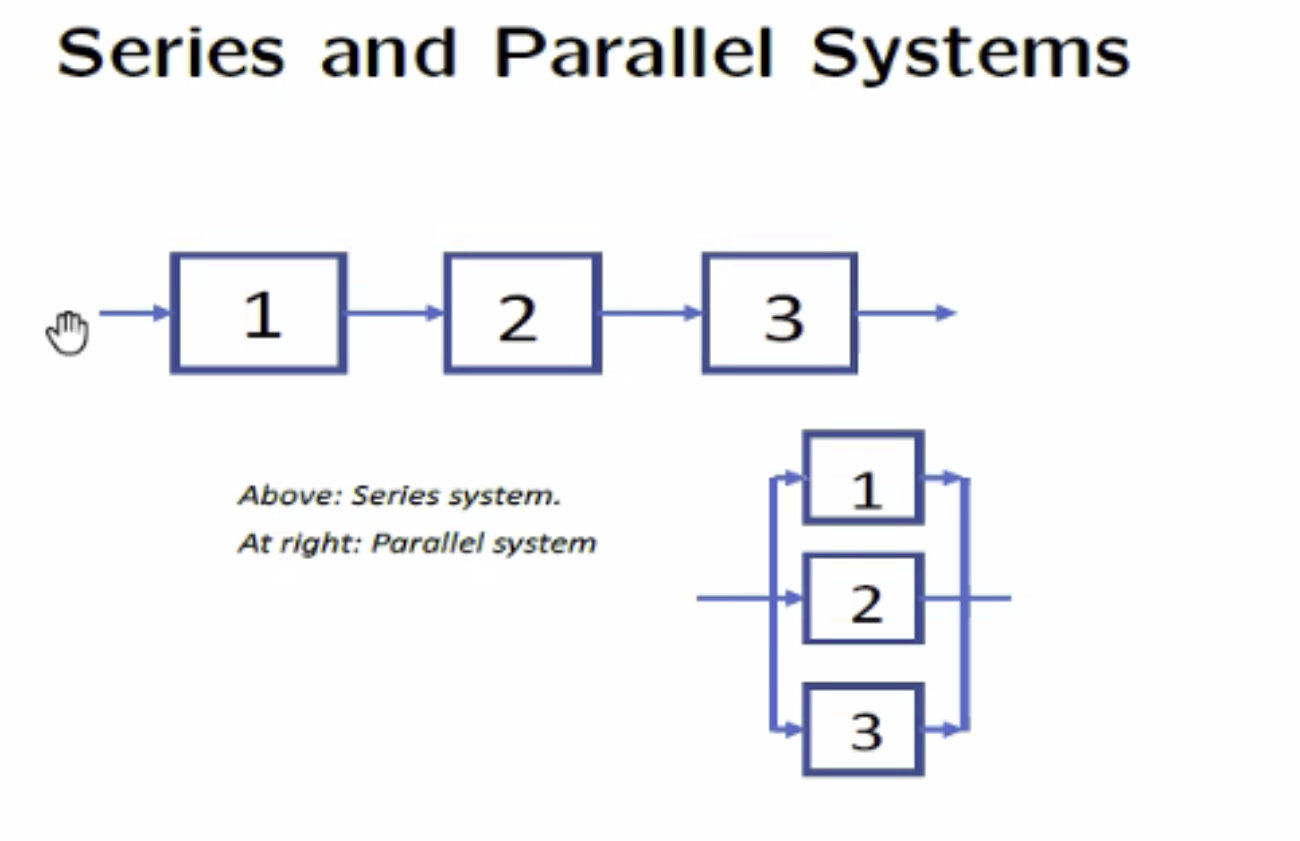
\includegraphics[scale=0.4]{media/wk2systems.png} \\%
\include{wk2/jul19}%
\include{wk2/jul20}%
\include{wk2/jul21}%
\include{wk2/jul22}%
\include{wk3/jul25}%
\include{wk3/jul26}%
\include{wk3/jul27}%
\include{wk3/jul28}%
\include{wk3/jul29}%
\include{wk4/aug1}%

\begin{thebibliography}{9}
  \bibitem{devore}
  Devore, J. L. (2016). Probability and Statistics for Engineering and the Sciences (9th edition). Cengage.
\end{thebibliography}
\end{document}

% Topics

% Data summary and visualization

% Sample mean, median, standard deviation

% *Sample quantiles, *box-plots

% (Scaled) relative-frequency histograms

% Probability

% Sample space, events, probability axioms

% Probabilities as limiting relative frequencies

% Counting techniques, equally likely outcomes

% Conditional probability, Bayes' Theorem

% Independent events

% *Probabilities as betting odds

% Discrete Random Variables

% Distributions of discrete random variables

% Probability mass function, distribution function

% Expected values, moments

% Binomial, hypergeometric, geometric, Poisson distributions

% Binomial as limit of hypergeometric distribution

% Poisson as limit of binomial distribution

% *Poisson process

% Continuous Random Variables

% Densities: probability as an integral

% Cumulative distribution, expectation, moments

% Quantiles for continuous rv's

% Uniform, exponential, normal distributions

% *Gamma function and gamma distribution

% *Other continuous distributions

% *Transformation of rv's (by smoothly invertible functions): distribution function and density

% *Simulation of pseudo-random variables of specified distribution (by applying inverse dist. func. to a uniform pseudo-random variable)

% Joint distributions, random sampling

% Bivariate rv's, joint (discrete) probability mass functions

% *Expectation of function of jointly distributed rv's

% *Joint and marginal densities

% *Correlation, *covariance

% Mutually independent rv's. Mean and variance of sums of independent rv's

% *Sums of rv's, laws of expectation

% Law of Large Numbers, Central Limit Theorem

% Connection between scaled histograms of random samples and probability density functions

% Point estimation

% Populations, statistics, parameters and sampling distributions

% Characteristics of estimators : consistency, accuracy as measured by mean square error, *unbiasedness

% Use of Central Limit Theorem to approximate sampling distributions and accuracy of estimators

% Method of moments estimator

% *Maximum likelihood estimator

% *Estimators as population characteristics of the empirical distribution

% Confidence intervals

% Large sample confidence intervals for means and proportions using Central Limit Theorem

% *Small sample confidence intervals for normal populations using Student's t distribution

% Confidence interval as decision procedure/hypothesis test

% Hypothesis Tests

% *Hypothesis testing definitions (Null and alternate hypotheses, Type I and II errors, significance level and power, p-values)

% *Tests for means and proportions in large samples, based on the Central Limit Theorem

% *Small sample tests for means of normal populations using Student's t distribution

% *Exact tests for proportions based on binomial distribution


% * = optional